\section{NUIssues}

\subsection{Rationale behind building an issue tracker}

NUI in software integration (obviously integrates with a different system, and provides valuable information about the current state of the company's project(s) and thus integrates with the company as well. Very easy to set up (many companies already have iPads hanging around – just get some more, or open a browser).

Motion controllers, gaze trackers, and brain trackers may be less interesting to use here (although Atlassian has been able to use brain power to move issues between swimlanes at a hackathon – or so they say.

The system is single-user, so inter-user task coupling has not been explicitly addressed, but it is possible to evolve the system to other forms of interfaces like touch walls or touch tables (or even just real-time updates for a project).

Inter-user task coupling (irrelevant because no two users will use the system at the same time – but could implement this with sockets so that both users will always know what the current status is)
  % TODO: Look into socket support for multi-user updates, in which case we probably move to lightly coupled tasks
  % TODO: figure out/discuss what type of coupling the tasks of updating an issue tracker are

\subsection{Scope}

Type: NUI, (not really) TUI, no VR/AR/MR. Obviously not a CLI because it has a GUI.

Form factor: designed only for iPad 1/2/Mini, but can easily write responsive CSS to support more types of devices (relevant for touch tables, smart boards, touch walls, smartphones). Hopefully keyboard is connected. Designed to be used when sitting down, although can be just opened (not interacted with) to grok the project's state on the move. Designed to be interacted with only when necessary and looked at when information is required

Could have built something native for better performance and complete control of the environment, but takes far too much time and was beside the concept we set out to prove.

Touch input: Fat fingers: no buttons (only large areas), large margins, everything can be dragged (no specific drag handles), may cause trouble with scrolling

\subsection{Sketching}

Figure \ref{figure:ipad-mockup} shows a simple initial mockup for the application's main functionality.

\begin{figure}[H]
    \centerline{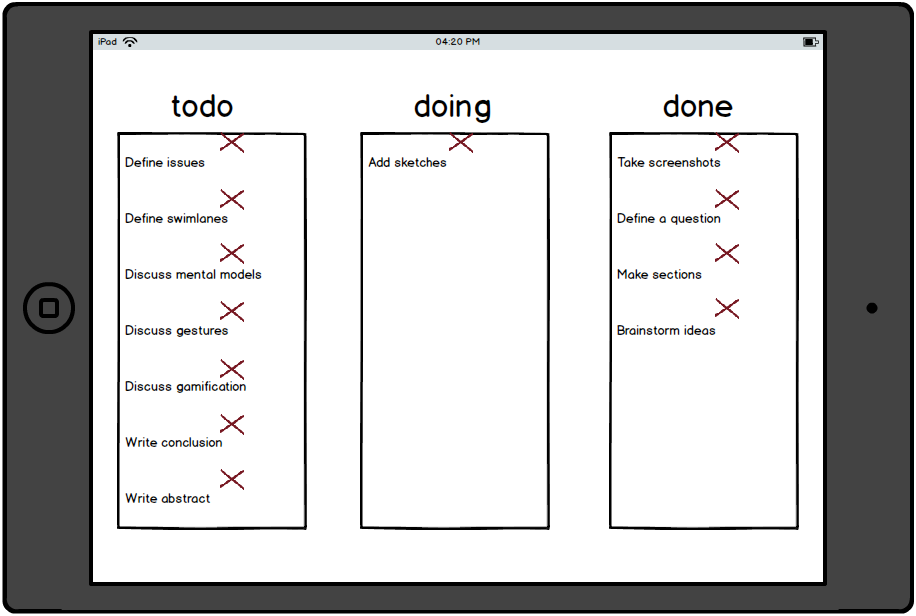
\includegraphics[scale=0.4]{images/mockup}}
    \caption{A simple mockup of the main functionality}   
    \label{figure:ipad-mockup}
\end{figure}

Figure \ref{figure:ipad-default-simple-screenshots} shows the implemented, much more refined and informative result.

\begin{figure}[H]
    \centerline{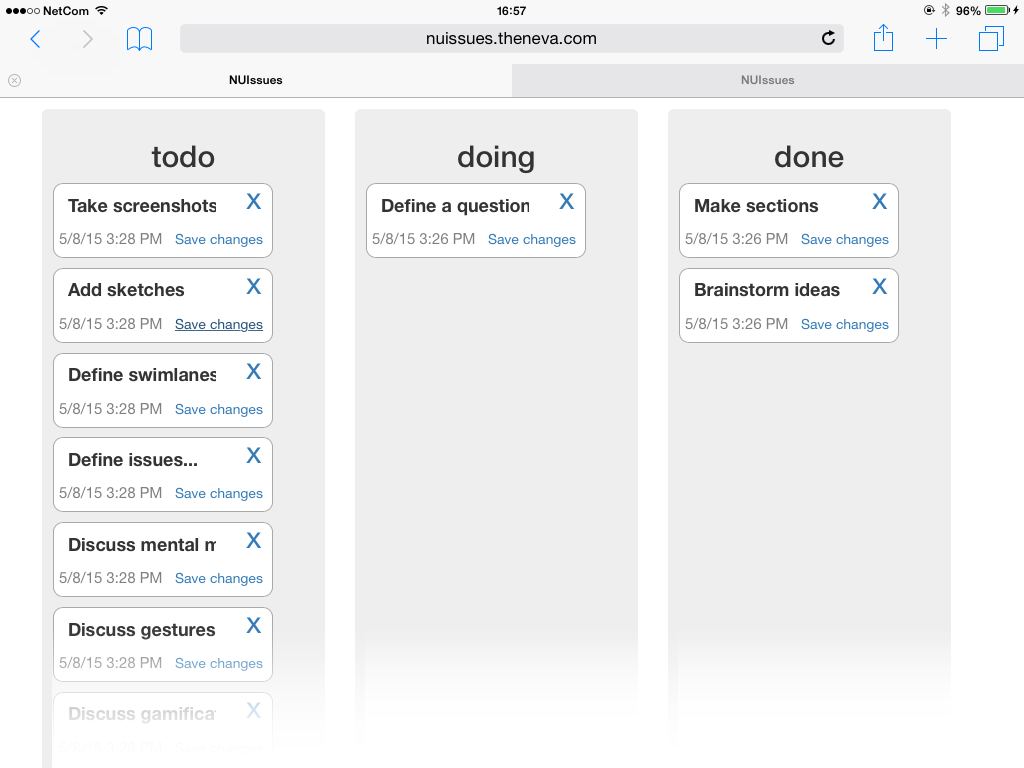
\includegraphics[scale=0.4]{images/nuissues-screenshots/01-default-all-swimlanes}}
    \caption{The system image for the main functionality}
    \label{figure:ipad-default-simple-screenshots}  
\end{figure}

% TODO: Cost/benefit discussion of different input types, what was NOT implemented

% TODO: Discuss fingerprint login (TUI!) and ethical issues with identifying someone/storing that type of information

Ethical problems: none in this application (except for security, duh), but certainly applicable % TODO: Digress into short discussion of ethical issues generally raised in NUI/Interactive Technologies contexts

Gamification: no users (and no points)\dots % TODO: look into and discuss how gamification could be utilised in a task tracker (public scoreboards, points, badges)

\subsection{Mental models}

Mental models: HCI Design: target system (duh), conceptual model (issue tracker with touch interface which supports only adding and moving/reordering issues), system image (the materialised version of the designer's mental model of the system), user's mental model of the system image (hopefully very close, but discuss this), designer's user model (hopefully very close, draw contrasts and use same metaphors/stuff as Trello, JIRA, Asana, ding.io, ServiceNow, Symfoni Notes, other issue trackers users have already used, and simple post-it note setups)

\subsection{Behaviour models}

Hick-Hyman Law: about reaction time when presented with a bunch of options, not really relevant as there are zero menus (for which the law is mostly being used)

Keystroke-level model (KLM): Key stroking only relevant when adding or editing issues, pointing relevant because the finger moves, homing time minimised because of large, responsive controls, drawing minimised (and destinations hinted), mental operator, system response operator (hello Heroku) % TODO look into mental operator and System Response operator

Motor behaviour models: descriptive models: (state 0: waiting for stimuli) -> <finger down on issue handle (entire issue)> -> ((state 1: dragging issue) -> <finger up above legal area> -> (state 2: releasing "dropping" issue) -> (state 0: waiting for stimuli)) OR (<finger up from text> -> (state 4: editing text) -> <tap "save changes" control> -> (state 0: waiting for stimuli))

\subsection{Development process}

Web client can be used by all types of devices (phones, tablets, touch tables, "smartboards", touch walls)

No specific SDKs have been used, although several frameworks are used:
\begin{itemize}
  \item AngularJS (front-end) with ng-sortable, bootstrap 3, custom CSS
  \item Node.js (back-end) with several components (Express web server, Mongoose ODM (could just as easily have used relations), body-parser)
  \item MongoDB document database (could just as easily have used relations for this simple use case)
  \item Potential: JWT (or just cookies): save data inside the token
\end{itemize}

\subsection{Known bugs}

\begin{itemize}
  \item It is nearly impossible to grab the bottommost issue that lies beneath the "fade out" overlay over the swimlane in a full swimlane
\end{itemize}
